\section{Results on the full DIPSER release (Q6)}
\label{sec:fullcorpus}

On the full release, folds group students unless a class is held out, and each success criterion was fixed before the run unless the experiment is marked exploratory.

\subsection{Replication of the fusion result}
\label{sec:fc-fusion}
The factorial grid was rerun with inputs standardised on the training fold, student-grouped folds and three seeds. The fusion result is replicated (Fig.~\ref{fig:full}): \fcFusionsAbove{} fusion configurations exceed the best single stream, which is again the face mesh (QWK \fcBestSingleQWK, 95\% CI \fcBestSingleCI). The best fusion obtains \fcBestFusionQWK, and the paired difference is \fcFusionDiff{} \fcFusionDiffCI{} ($p=\fcFusionP$). The data are thus compatible with a small difference in either direction, but not with a fusion gain larger than about 0.02.

All streams are considerably weaker than on the slice. On the slice, 59\% of the label variance lies between the 20 students, so that a model can score by recognising which students tend to be rated as attentive; this is no longer the case with \fcPersons{} students (Section~\ref{sec:fc-labels}). Two further measurements indicate what the models capture. First, the agreement with changes \emph{within} a student-session is small (correlation $\le\fcWithinSessionMax$ for every stream). Second, no stream significantly outperforms a control model that is trained on the label of a \emph{classmate} at the same moment (closest: the \fcClassmateStream{} stream, $p=\fcClassmateP$; dashed line in Fig.~\ref{fig:full}). The streams of a student therefore carry mainly information about what the class is doing, and little that is specific to the student.

\begin{figure}[!t]
\centering
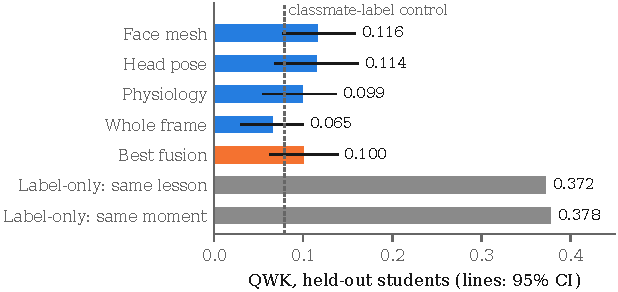
\includegraphics[width=\columnwidth]{figures/fig_full_release.pdf}
\caption{Full DIPSER release, held-out students. QWK of the best configuration of each single stream and of the best fusion, with 95\% bootstrap intervals over students. Grey bars: label-only references that use the labels of the other students (not deployable). Dashed line: highest QWK of the classmate-label controls.}
\label{fig:full}
\end{figure}

\subsection{Structure of the labels}
\label{sec:fc-labels}
Of the label variance, \fcSharePerson\% lies between students, \fcShareClass\% between class sessions and \fcShareSession\% between student-sessions. In this dataset the rated attention is thus mainly a property of a lesson, and of a student within that lesson, rather than a stable trait of the student; the nine sessions of a group are nine different activities. Two label-only references quantify this structure. They use no sensor, and they cannot be deployed because they read the labels of other students. The mean label of the other students in the same class session yields QWK \fcExpPrior, and the labels of the other students at the same 4-s moment yield \fcMomentPrior. Both are about three times the best sensor model (Fig.~\ref{fig:full}).

\subsection{Attempts to improve the sensor model}
\label{sec:fc-limits}
Table~\ref{tab:fc-tests} summarises the attempts; every comparison is paired on the same students.

\textbf{Search and higher-order moments.} A Bayesian search (tree-structured Parzen estimator) over the streams, the moment orders, the model family (multilayer perceptron or gradient-boosted trees), the model size, the learning rate, the class weights and the head was evaluated on a fixed split with 13 held-out test students, scored once with three seeds. It reaches \fcSearchPaperAcc\% test accuracy against a majority rate of \fcSearchMajority\%. Moments re-extracted at higher orders ($24\times24$ in space, 12 in time) give \fcSearchRichAcc\%, a difference that is not significant, and the search itself selects low orders (6--8 in space, 5--7 in time).

\textbf{Face crop and moment families.}
\label{sec:fc-crop}
Because the image stream is the whole webcam frame, we constructed a face crop from the per-frame face box of the DIPSER metadata (square, 10\% margin). Frames without a detected face become blank images, so that the visibility of the face is itself encoded. The crop was described with five discrete orthogonal moment families: Tchebichef, Hahn ($\alpha=\beta=4$) and Krawtchouk centred on the face, on the eyes and on the mouth. Unlike Tchebichef moments, Hahn and Krawtchouk moments are local and concentrate on a region of the image. A self-test confirmed that the whole-frame Tchebichef moments recomputed by the new pipeline equal the original features in all 35{,}374 comparable windows. The crop raises accuracy by \fcCropAccGain{} points \fcCropAccCI{} over the whole frame, but it does not significantly change QWK. No family outperforms Tchebichef under the predefined rule, which required a Holm-corrected gain in both an accuracy-tuned and a QWK-tuned search; the best family, Hahn, gains $+0.036$ in the latter (Holm $p=0.13$) and $+0.010$ in the former.

\textbf{Temporal and class context.} Because the raters mark change points, consecutive windows usually share a label. A causal recurrent model (GRU) that reads the preceding windows of the student nevertheless leaves QWK unchanged (\fcCtxNoneQWK{} for isolated windows, \fcCtxGruQWK{} with the past, and \fcCtxBiQWK{} for an offline bidirectional model). Adding the sensor features of the other students at the same moment, without their labels, does not significantly improve QWK on a class unseen during training (\fcLogoOwnQWK{} to \fcLogoClassQWK).

\textbf{Pretrained face encoders.} To test whether the moment front-end is the limiting factor, we added frozen pretrained encoders of the face crop to the sensor features (mean and standard deviation of the embeddings of up to eight crops per window): ResNet-18~\cite{he2016deep}, DINOv2~\cite{oquab2024dinov2} and an expression network trained for emotion and engagement~\cite{savchenko2022hsemotion}. On a held-out class the sensor features give \fcEncBaseAcc\% accuracy and QWK \fcEncBaseQWK; adding an encoder gives QWK \fcEncResQWK, \fcEncDinoQWK{} and \fcEncExprQWK{} respectively, none significantly different. The third encoder was added after the results of the first two were known.

\begin{table*}[!t]
\centering
\caption{Attempts to improve performance on the full release. $\Delta$QWK: second condition minus first, paired on the same students (bootstrap over students, 95\% CI); two-sided $p$, Holm-adjusted within the moment families and within the encoders. Phase: label of the experiment in the released plan. Rule: pre-decl., criterion fixed before the run; explor., no predefined criterion.}
\label{tab:fc-tests}
\small
\setlength{\tabcolsep}{2.5pt}
\begin{tabular}{lcccccc}
\toprule
Comparison & Phase & Rule & $\Delta$QWK & 95\% CI & $p$ & Improves \\
\midrule
\csname @@input\endcsname tables/fullcorpus_tests.tex
\bottomrule
\end{tabular}
\end{table*}

\subsection{Tracking with sparse label probes}
\label{sec:fc-probe}
Since sensors alone fail, we tested a different task, in which some labels are available at test time. The consensus label of a student is revealed at a probe every 32\,s, 1\,min or 2.5\,min, and the windows in between are predicted causally. The model reads the sensors of the current window and of the last probe window, the labels of the last two probes and the time since the last probe; it never reads a later label or the label of another student. Evaluation is on a held-out class, with gradient-boosted trees, three seeds and all \fcWindows{} windows (majority rate \fcMajorityAll\%); the model settings and the decision rules were fixed in advance.

Table~\ref{tab:fc-probe} and Fig.~\ref{fig:probe} compare three predictors: repeating the last probe (persistence), a model of the probe labels alone, and the same model with sensors. With a probe every 32\,s the full model reaches \fcProbeHalfAcc\% accuracy and QWK \fcProbeHalfQWK, and with one probe per minute \fcProbeOneAcc\% and \fcProbeOneQWK, against \fcSensorsOnlyAcc\% and \fcSensorsOnlyQWK{} for sensors alone. Persistence, however, already obtains \fcPersistHalfAcc\% and \fcPersistHalfQWK{} (\fcPersistOneAcc\% and \fcPersistOneQWK{} per minute). The sensors add between 1 and 3 points of accuracy, with confidence intervals that exclude zero, and no QWK. This is consistent with a report on self-rated attention in video learning, in which carrying the last rating forward gives a lower error than sensor models when forecasting the next ratings~\cite{leng2026edugage}.

The probe above is the consensus label. With the self-report of the student as the probe and the expert labellers as the target, persistence gives only \fcSelfPersistHalfAcc\% accuracy and QWK \fcSelfPersistHalfQWK{} at 32\,s, because the self-reports agree poorly with the labellers (QWK \fcSelfExtQWK). The self-reports of DIPSER are given retrospectively~\cite{marquezcarpintero2025dipser}, which may contribute to this disagreement. The tracking result therefore requires probes of observer quality.

\begin{figure}[!t]
\centering
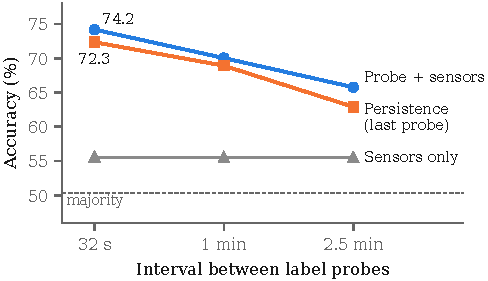
\includegraphics[width=\columnwidth]{figures/fig_probe.pdf}
\caption{Sparse-probe tracking on a held-out class: accuracy on the windows between probes as a function of the probe interval (three seeds). The gap between the two upper curves is the contribution of the sensors.}
\label{fig:probe}
\end{figure}

\begin{table*}[!t]
\centering
\caption{Sparse-probe tracking on a held-out class (accuracy\,\% / QWK on the windows between probes, three seeds). Gain: probe + sensors minus persistence, bootstrap over students, 95\% CI.}
\label{tab:fc-probe}
\small
\setlength{\tabcolsep}{3pt}
\begin{tabular}{lccccc}
\toprule
Probe every & Persistence & Probe model & Probe + sensors & Acc.\ gain (points) & QWK gain \\
\midrule
\csname @@input\endcsname tables/fullcorpus_probe.tex
\bottomrule
\end{tabular}
\end{table*}

\subsection{Effect of the evaluation protocol}
\label{sec:fc-protocol}
Table~\ref{tab:fc-protocol} and Fig.~\ref{fig:protocol} report two experiments, each of which keeps the model fixed and changes only what the test set shares with the training set.

In the first, model A is evaluated on random windows and on held-out students. With random windows, the windows of a student fall on both sides of the split, often seconds apart, and the model obtains \fcLeakRandAcc\% accuracy and QWK \fcLeakRandQWK. With whole students held out it obtains \fcLeakPersonAcc\% and \fcLeakPersonQWK{} (majority rate \fcMajority\%).

In the second, model B is evaluated on held-out students and on a held-out class. Holding out a class lowers QWK from \fcPgOwnQWK{} to \fcLogoOwnQWK{} (paired difference for seed 0: \fcLogoDrop{} \fcLogoDropCI), which indicates that part of what is learned is specific to the lessons seen in training. The effect is largest when class features are used (model B$'$). With students held out, these features appear to raise QWK from \fcPgOwnQWK{} to \fcPgClassQWK{} (\fcLeakClassDiff{} \fcLeakClassCI): the labels of the classmates at the same moment are in the training set, and the class features allow the model to retrieve them. On an unseen class this gain disappears.

Across the splits that hold out students or classes, accuracy remains within a few points of the majority rate (\fcLogoOwnAcc--\fcLeakPersonAcc\% against \fcMajority\%), whereas QWK decreases four-fold from random windows to a held-out class.

\begin{figure}[!t]
\centering
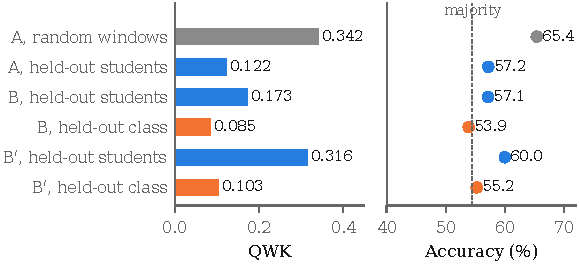
\includegraphics[width=\columnwidth]{figures/fig_protocol.pdf}
\caption{The same models under different splits (full release, complete windows). A: model of the hyper-parameter search; B: window-level perceptron on all streams including the face crop; B$'$: B with the sensor features of the classmates. Dashed line: majority accuracy.}
\label{fig:protocol}
\end{figure}

\begin{table*}[!t]
\centering
\caption{The same model under different splits (full release, complete windows, pooled out-of-fold predictions, majority accuracy \fcMajority\%). A: model of the hyper-parameter search (three seeds); B: window-level perceptron on all streams including the face crop (three seeds; student-grouped: one seed); B$'$: B with the sensor features of the classmates.}
\label{tab:fc-protocol}
\small
\setlength{\tabcolsep}{3pt}
\begin{tabular}{lllcc}
\toprule
Model & Split & Shared with the training set & Acc.\,\% & QWK \\
\midrule
\csname @@input\endcsname tables/fullcorpus_protocol.tex
\bottomrule
\end{tabular}
\end{table*}
